\chapter{Introduction} \label{ch:intro}

Welcome to Dynare\index{Dynare}! \\

\section{About this Guide}
This User Guide aims to help you master Dynare's main functionalities, from getting started to implementing advanced features. To do so, this Guide is structured around examples and offers practical advice. To root this understanding more deeply, though, this Guide also gives some background on Dynare's algorithms, methodologies and underlying theory. Thus, a secondary function of this Guide is to serve as a basic primer on DSGE model solving and estimation. \\

This User Guide is written mainly for new users, although an intermediate user may find it helpful to expand his or her capabilities into new areas of functionality. More importantly, the Guide is written mainly for an \textbf{advanced economist} - like a professor, graduate student or central banker - needing a powerful program to support his or her research activities in a variety of fields. The coder or programmer, on the one hand, or the specialist of computational economics, on the other, may not find this Guide sufficiently detailed. \\

With the hope of making you feel comfortable with using Dynare, this Guide will focus on the most common or useful features of the program. Depth will therefore supercede breadth; the idea is to get you to use 90\% of the program and then tell you where else to look if you're interested in fine tuning or advanced customization.\\

As much as possible, this Guide will introduce the various Dynare commands and features through illustrative examples. You will also find the marker \textbf{\textsf{TIP!}} throughout the Guide, emphasizing advice you will hopefully find useful to work more efficiently with Dynare; often, these are drawn from past users' frequently asked questions. In this same spirit, you will also find \textbf{boxes} throughout this Guide relating particularly important information, or giving you some background to better grasp a new feature.\\

\section{What is Dynare?}
Before we dive into the multitude of ``trees'' making up the features, commands and options of Dynare, let's have a look at the ``woods'' from the top \ldots just what is Dynare? Dynare is a powerful and highly customizable engine, with an intuitive front-end interface, to solve, simulate and estimate DSGE models. In slightly less flowery words, it is a pre-processor and a collection of Matlab routines that has the advantages of reading DSGE model equations written almost as in an academic paper. \\

\begin{figure} \label{fig:dyn}
\begin{center} 
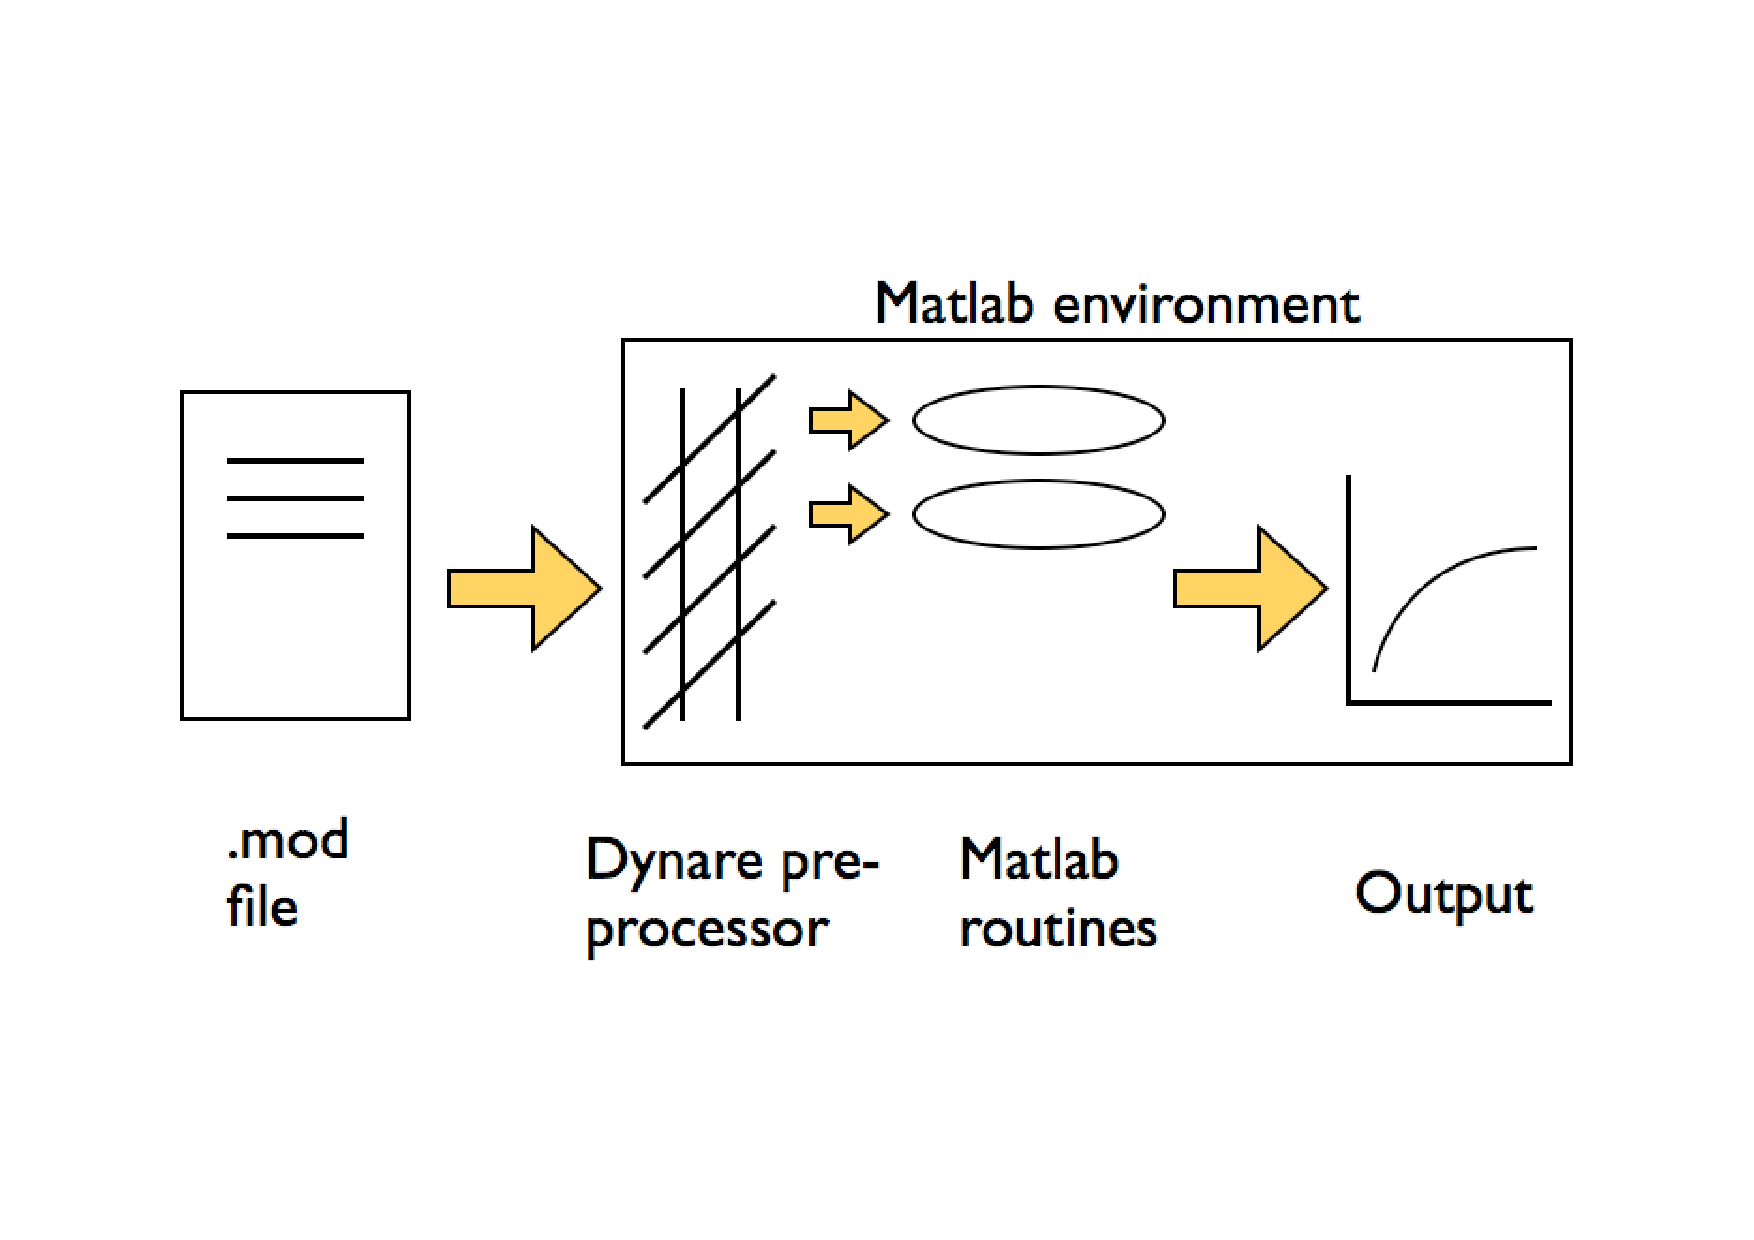
\includegraphics[width=1.0\textwidth]{P_DynareStruct2} 
\end{center} 
\caption[Dynare, a bird's eyeview]{The .mod file being read by the Dynare pre-processor, which then calls up the relevant Matlab routines to carry out the desired operations and display the results.} 
\end{figure}
Figure \ref{fig:dyn} gives you an overview of the way Dynare works. Basically, the model and its related attributes, like a shock structure for instance, is written in a .mod file in any editor of your choice. That file is then called from Matlab. This initiates the Dynare pre-processor which reads the file and calls the relevant Matlab routines to either solve or estimate the model. Finally, results are presented in Matlab. Each of these steps will become clear as you read through the User Guide, but for now, it may be helpful to summarize what \textbf{Dynare is able to do}:
\begin{itemize}
\item compute the steady state of a model
\item compute the solution of deterministic models
\item compute the first and second order approximation to solutions of stochastic models 
\item estimate parameters of DSGE models using either a maximum likelihood or a Bayesian approach
\item compute optimal policies in linear-quadratic models
\end{itemize}

This \textbf{User Guide is structured} according to each of Dynare's capabilities mentioned above. First, though, chapter \ref{ch:inst} outlines system requirements and installation procedure. But then, Chapter \ref{ch:solbase} deals with the basics of model solution and simulation, using a simple RBC example, in both a stochastic and deterministic context. Chapter \ref{ch:estbase} moves on to the fundamentals of model estimation, mainly using Bayesian\index{Bayesian} techniques which it tries to motivate by listing their advantages with respect to other estimation methodologies. Once you have read these two chapters, you will already know the crux of Dynare's functionality and will (hopefull!) feel comfortable moving on to using Dynare for your own work. The following two chapters, chapter \ref{ch:soladv} and \ref{ch:estadv}, cover more advanced features for model solution and estimation respectively, and shed some light on what really happens behind the scenes of Dynare computations. Finally, chapter \ref{ch:ramsey} introduces Dynare's capacity to compute optimal Ramsey policies. \\

\section{Additional sources of help}
All in all, this User Guide tries to be as complete and thorough as possible. But you will certainly want to browse other material for help, as you learn about new features, struggle with adapting examples to your own work, and yearn to ask that one question whose answer seems to exist no-where. At your disposal, you have the following additional sources of help:
\begin{itemize}
\item The Reference Manual (**add link): this manual covers all Dynare commands, giving a clear definition and explanation of usage for each. The User Guide will often introduce you to a command in a rather loose manner (mainly through examples); so reading corresponding command descriptions in the Reference Manual is a good idea to cover all relevant details. 
\item \href{http://www.cepremap.cnrs.fr/juillard/mambo/index.php?option=com_content&task=category&sectionid=11&id=96&Itemid=89}{Official online examples}: the Dynare website includes other examples - usually well documented - of .mod files covering models and methodologies introduced in recent papers. 
\item \href{http://www.cepremap.cnrs.fr/juillard/mambo/index.php?option=com_forum&Itemid=95&page=viewforum&f=2&sid=10290a11eb7a48243971159f5b86f83e}{Open online examples}: this page lists .mod files from various users covering a wide variety of examples. 
\item \href{http://www.cepremap.cnrs.fr/juillard/mambo/index.php?option=com_forum&Itemid=95&page=viewforum&f=1}{Dynare forums}: this lively online discussion forum allows you to ask your questions openly and read threads from others who might have run into similar difficulties. 
\item \href{http://www.cepremap.cnrs.fr/juillard/mambo/index.php?option=com_content&task=section&id=3&Itemid=40}{Frequently Asked Questions} (FAQ): this section of the Dynare site emphasizes a few of the most popular questions users ask in the forums. 
\item \href{http://www.dsge.net}{DSGE.net}: this website is a resource for all scholars working in the field of DSGE modeling. Besides allowing you to stay up to date with the most recent papers and possibly make new contacts, it conveniently lists all related conferences, workshops and seminars that may be of interest. 
\end{itemize}

\section{Nomenclature}
To end this introduction and avoid confusion in what follows, it is worthwhile to agree on a few \textbf{definitions of terms}. Many of these are shared with the Reference Manual. 
\begin{itemize}
\item \textbf{Integer} indicates an integer number
\item \textbf{Double} indicates a double precision number. The following syntaxes are valid: 1.1e3, 1.1E3, 1.1d3, 1.1D3
\item \textbf{Expression} indicates a mathematical expression valid in the underlying language (e.g. Matlab)
\item \textbf{Variable name} indicates a variable name starting with an alphabetical character and cannot contain ()+ --*/ $\hat{}$ =!;:@\# or characters with accents
\item \textbf{Parameter name} indicates a parameter name starting with an alphabetical character and cannot contain any of the above mentioned characters. 
\item \textbf{Filename} indicates a file name valid in your operating system
\item \textbf{Command} is a word with a specific meaning in Dynare
\item \textbf{Options} or optional arguments for a command are listed in square \mbox{[ ]} unless otherwise noted
\item \textbf{\texttt{Typewritten text}} indicates text that should appear in Dynare code

\end{itemize}


 

